\subsection{L'ipotesi di De Broglie}
Il modello di Bohr doveva quindi essere superato. Per fare ciò si suppose che l'energia e la massa fossero aspetti diversi (e ciò significa che caratteristiche ondulatorie e corpuscolari sono entrambe presenti) in tutte le radiazioni ed i corpi.

Equazione di Einstein (1915) $E=mc^2$.

L'effetto fotoelettrico mostrò che la luce, considerata di solito come onda, può anche avere proprietà corpuscolari sebbene senza massa. Nel 1924 De Broglie per primo parlò di dualismo onda-particella, affermando che le particelle elementari (quindi anche gli elettroni) avessero proprietà ondulatorie, in analogia alle radiazioni. In altre parole suppose che gli elettroni potessero dar luogo a fenomeni ondulatori. Egli partì dalla relazione di Planck $E=h\nu$ e ipotizzò che la frequenza sia inversamente proporzionale alla lunghezza d'onda con la relazione $\nu=c/\lambda$. Sostituendo
$$E=h\frac{c}{\lambda}$$
La quantità di moto è $p=mv$, per la velocità della luce $p=mc$, da cui
$$E=mc \cdot c=pc$$
Uguagliando le due formule dell'energia
$$pc=h\frac{c}{\lambda} \implies p=\frac{h}{\lambda}$$
Cioè la quantità di moto è inversamente proporzionale alla lunghezza d'onda, il che implica che lo sia anche la massa. Questa è l'ipotesi di De Broglie.

A favore di questa ipotesi, sperimentalmente si osserva che per oggetti microscopici le lunghezze d'onda sono ragionevolmente simili alle dimensioni dell'oggetto stesso e con quelle delle distanze interatomiche, e le proprietà corpuscolari diventano meno evidenti in quanto prendono il sopravvento quelle ondulatorie. Per oggetti macroscopici invece le lunghezze d'onda diventano estremamente piccole, per cui le proprietà ondulatorie associate a tali oggetti non sono evidenti alla nostra esperienza.

Se quindi voglio studiare il comportamento di un elettrone all'interno dell'atomo, più che immmaginarlo come un corpo si devono studiare le sue proprietà ondulatorie: devo immaginare che sia un'onda elettromagnetica.
\subsection{L'esperimento di Davisson e Germer}
La conferma sperimentale all'ipotesi di De Broglie arrivò nel 1927 con l'esperimento di Davisson e Germer, che compivano studi di diffrazione. Loro volevano studiare la diffrazione dei raggi X inviati ad un cristallo di Nichel, solo che per errore inviarono un fascio di elettroni. Inizialmente non si accorsero di questo errore, perché la diffrazione ottenuta era la stessa di quella che si sarebbe ottenuta coi raggi X.
Questo esperimento pose le basi per lo studio della funzione d'onda per l'elettrone inteso come radiazione elettromagnetica \footnote{Ciò implicherà che l'elettrone non è più localizzato: è in tutti i posti perché la radiazione copre tutta lo spazio, infatti si passa dal concetto di orbita a quello di orbitale.}.

Considerando l'elettrone come radiazione elettromagnetica si riesce facilmente a spiegare gli spettri di emissione: fornendo energia ad un elettrone esso si sposta da uno stato ad un altro (emissione $\rightarrow$ righe). Se invece forniamo tantissima energia l'elettrone riesce a sfuggire al nucleo e manifesta caratteristiche corpuscolari.
%ora dice una roba sul fatto che dentro l'atomo l'elettrone sente un campo elettrico non lo so quanto sia giusto

Elettrone dentro l'atomo $\rightarrow$ natura ondulatoria.

Elettrone emesso $\rightarrow$ natura corpuscolare.
\subsection{Finalmente sta benedetta equazione}
Serve ora una funzione d'onda.

Si parte dall'energia dell'elettrone all'interno di un atomo:
$$E=E_{cin} + E_{pot}=\frac{1}{2}m_ev^2 - \frac{e^2}{r}$$
Inoltre
$$p=mv \implies p^2=m^2v^2 \implies mv^2=\frac{p^2}{m}$$
Ne segue
$$E=\frac{p^2}{2m} - \frac{e^2}{r}$$
Mentre in meccanica classica p è un vettore, in quella ondulatoria è un operatore, che si esprime come
$$p=\frac{h}{2\pi \text{i}}\frac{d}{dx}\implies p^2=-\frac{h^2}{4\pi^2}\frac{d^2}{dx^2}$$
$$E=-\frac{h^2}{8\pi^2m}\frac{d^2}{dx^2} -\frac{e^2}{r}$$
Chiamata $\Psi$ la funzione d'onda che ci serve per studiare l'elettrone, se la moltiplico per l'energia E ottengo l'energia totale del sistema. Quest'espressione si chiama "Hamiltoniana di $\Psi$"
$$H\Psi=E\Psi \rightarrow \biggl(-\frac{h^2}{8\pi^2m}\frac{d^2}{dx^2} -\frac{e^2}{r}\biggr)\Psi=E\Psi$$
Nello spazio l'equazione diventa
$$-\frac{h^2}{8\pi^2m}\biggl( \frac{\partial^2\Psi}{\partial x^2}+\frac{\partial^2\Psi}{\partial y^2}+\frac{\partial^2\Psi}{\partial z^2}\biggr) -\frac{e^2}{r}\Psi =E\Psi$$
In forma contratta
$$H\Psi=E\Psi \qquad \textbf{Equazione di Schrödinger}$$
Questa è l'equazione d'onda per l'elettrone. Essa mette in relazione la funzione d'onda con la sue energia, ed essa prende il nome di "equazione agli autovalori", nel senso che possiamo immaginare l'energia dell'elettrone come data dalla combinazione lineare delle varie funzioni d'onda (che costituiscono le autofunzioni) moltiplicate per le rispettive energie (che costituiscono gli autovalori).

Tuttavia questa equazione ammette un numero infinito di soluzioni, ma noi consideriamo solo quelle che hanno significato fisico e pertanto imponiamo due condizioni a contorno affinché restringiamo l'insieme delle soluzioni:
\begin{itemize}
  \item  Le funzioni e le loro derivate prime devono essere finite, continue e ad un solo valore in ogni punto dello spazio;
  \item Condizione di normalizzazione: mentre la funzione d'onda $\Psi$ non ha significato, il suo quadrato $\Psi^2$ rappresenta la probabilità di trovare l'elettrone attorno al nucleo. Essa deve corrispondere al 100\%, cioè devo avere certezza di ragionare su un volume dello spazio in cui la probabilità di trovare l'elettrone è totale. Questa condizione si scrive integrando su tutto lo spazio:
  $$\iiint \Psi^2dV=1$$
  Il significato di tale integrale è che per avere il 100\% di probabilità di trovare l'elettrone dovremmo considerare volumi infiniti. Nella pratica si scende al 95\% di probabilità, che è ragionevole in quanto per tale valore il volume diventa piccolissimo. Ciò significa che l'elettrone ha un'alta probabilità di trovarsi vicino al nucleo, e man mano che ci sia allontana da esso la probabilità crolla drasticamente, per cui l'errore commesso nel considerare solo un volume piccolo attorno al nucleo è accettabile. Attenzione però: l'elettrone occupa interamente il volume considerato e in ogni punto la probabilità di trovarlo è la stessa.
\end{itemize}
La funzione d'onda viene chiamata \textbf{orbitale}. Esso è come la casa di una persona: se una persona esiste potrebbe avere una casa, ma se non esiste sicuramente non esiste nemmeno casa sua. L'orbitale è una regione dello spazio dove può esserci l'elettrone: se c'è riempie tutto quello spazio, non è in un punto solo. Ecco perché era sbagliata l'orbita di Bohr in cui si muovevano gli elettroni. 

In un atomo si hanno tante funzioni d'onda quanti sono gli elettroni (infatti più che di orbitali si parla di spin-orbitali).
\subsection{I numeri quantici}
Le soluzioni dell'equazione di Schrödinger a cui sono state applicate le condizioni a contorno sono legate a 4 numeri interi detti numeri quantici. Tali numeri sono gli stessi che erano stati imposti nei calcoli sia nell'equazione di Planck che nel modello atomico di Bohr, solo che adesso vengono fuori dalla risoluzione di tale equazione.

Reminder: I risultati che seguono valgono solo per l'atomo di idrogeno, perché è solo per esso che siamo in grado di calcolare le soluzioni esatte dell'equazione di Schrödinger, poiché con più elettroni nell'equazione figura un termine misto di interazione di energia potenziale repulsiva tra gli elettroni, il quale non permette di separare le variabili e di fatto l'equazione non può essere risolta. Pertanto per gli altri atomi faremo approssimazioni.

I numeri quantici permettono di classificare le diverse funzioni d'onda. Essi sono 4 e si indicano con \textbf{n}, \textbf{l}, \textbf{m} e \textbf{s}:
\begin{itemize}
  \item \textbf{n} è il numero quantico principale, quello che quantizza l'energia del sistema e determina la \textbf{dimensione} di un orbitale.
  Può assumere tutti i valori interi positivi:
  $${n=1,2,...,\infty}$$
  $n$ può assumere valori molto grandi perché per avere certezza matematica di trovare l'elettrone in quell'orbitale dobbiamo integrare in tutto lo spazio.
  \item \textbf{l} è il numero quantico che quantizza il momento angolare. Può assumere tutti i valori compresi tra 0 e $n$-1:
  $$l=0,1,...,n-1$$
  ES
  $$n=3 \implies l=0,1,2$$
  $$n=5 \implies l=0,1,2,3,4$$
  Esso "dà" la forma dell'orbitale.
  \item \textbf{m} è il numero quantico magnetico. Esso quantizza il momento magnetico dell'elettrone e determina l'\textbf{orientamento} dell'orbitale. Se infatti per un momento torniamo all'idea di Bohr, l'elettrone si muove attorno al nucleo, ed essendo una particella carica in movimento genererà un campo magnetico e un conseguente momento magnetico.
  
  Esso può assumere valori che dipendono da l e determina la \textbf{forma} dell'orbitale. in particolare assume tutti i valori compresi tra $-l$ e $l$, incluso lo zero:
  $$m=-l,-l+1,...,-2,-1,0,1,2,...,l-1,l$$
  ES 
  $$n=3 \implies l=0,1,2$$
  $$l=0 \implies m=0$$
  $$l=1 \implies m=-1,0,1$$
  $$l=2 \implies m=-2,-1,0,1,2$$
  \item \textbf{s} è il numero quantico di spin. Esso ci dà informazioni sulla rotazione oraria o antioraria dell'elettrone attorno a se stesso. Può assumere valore pari $\pm\frac{1}{2}$
  $$s=\frac{1}{2}\implies \text{rotazione oraria}$$
  $$s=-\frac{1}{2}\implies \text{rotazione antioraria}$$
\end{itemize}

Per un atomo vale poi il \textbf{Principio di esclusione di Pauli}: in un orbitale non possono stare più di due elettroni, e se ce ne sono due devono avere spin opposto.

Un modo più completo per enunciarlo è il seguente:

"\textit{In un atomo non possono esistere due elettroni che abbiano la stessa sequenza di numeri quantici.}"

In realtà stiamo dicendo la stessa cosa perché elettroni che stanno su orbitali diversi hanno i primi tre numeri quantici diversi, mentre elettroni che stanno nello stesso orbitale hanno i primi tre numeri quantici uguali ma spin opposto.\\

Poiché tali numeri nascono da esigenze matematiche e non sono imposti, è chiaro che la funzione d'onda dipende da essi: $\Psi\rightarrow\Psi(n,l,m,s)$.

\subsection{Il simbolismo degli orbitali}
Al posto dei numeri quantici si usa un simbolismo che li riassume:
\begin{itemize}
\item Se l=0 si parla di orbitale s.

In questo caso può essere solo m=0 e quindi si ha un solo tipo di orbitale s;
\item Se l=1 si parla di orbitale p

In questo caso m=-1, 0, 1 per cui ci sono tre tipi di orbitali p: $p_x, \; p_y \; \text{e} \; p_z$;
\item Se l=2 si parla di orbitale d

In questo caso m=-2, -1, 0, 1, 2 per cui ci sono cinque tipi di orbitali d:

$d_{z^2}, \; d_{x^2-y^2}, \; d_{xy}, \; d_{xz} \; \text{e} \; d_{yz}$
\end{itemize}  
Tale classificazione vale $\forall n$, quindi avremo orbitale 1s, 2s, 3s ecc; orbitali 2p, 3p ecc.; orbitali 3d ecc. 

\subsection{Il principio di indeterminazione di Heisenberg}
Il concetto di orbita quindi si perde, perché si è intuito che l'elettrone è interamente diffuso in una regione dello spazio. Da ciò segue che non abbiamo modo di conoscere con esattezza la sua posizione, e dunque si parla di probabilità (analogamente avviene per la velocità).
Si introduce quindi il principio\footnote{È un principio perché non può essere dimostrato, ma che viene assunto vero in quanto non si è mai osservato un fenomeno che lo contraddicesse.} di indeterminazione di Heisenberg. Esso è legato alla conoscenza probabilistica di alcune grandezze ed è enunciato così:

"Il prodotto tra l'indeterminazione sulla posizione $\Delta x$ e quella sulla quantità di moto $\Delta p$ deve sempre essere maggiore o uguale di $h/4\pi$"
$$\Delta x \Delta p \geq \frac{h}{4\pi}$$
Tale principio ci dice che se riusciamo a determinare la posizione con precisione elevata (il che significa commettere un errore piccolo), inevitabilmente crescerà l'errore che commetteremo sulla quantità di moto. Chiaramente vale anche il viceversa.

Può essere riscritto anche come
$$\Delta x \Delta v \geq \frac{\hbar}{2m} \qquad \hbar=\frac{h}{2\pi}$$
\begin{itemize}
  \item Per particelle macroscopiche la massa è grande, perciò $\hbar/2m$ è piccolo e di conseguenza possiamo conoscere con buona precisione la loro velocità e posizione;
  \item Per particelle microscopiche la massa è piccola, perciò $\hbar/2m$ è molto grande e di conseguenza il prodotto tra le indeterminazioni d velocità e posizione, il che significa che se tentiamo di minimizzare uno dei due l'altro cresce di molto.
\end{itemize}
\newpage
\subsection{La geometria degli orbitali}
Le sequenze di numeri quantici ci danno energia e forma dell'orbitale (nel senso che ci dicono come varia la probabilità di trovare l'elettrone attorno al nucleo).

Per l'atomo di idrogeno vale quanto Bohr aveva già affermato, cioè che l'energia è quantizzata da $n$. Egli infatti affermava (col raggio di Bohr) che all'aumentare di $n$ aumenta anche la distanza media elettrone-nucleo, cioè il limite esterno dell'orbitale.

Infatti all'aumentare di $n$ l'energia dell'elettrone aumenta in valore assoluto (l'energia di uno stato legato è sempre negativa), e man mano che l'elettrone si allontana dall'atomo tende a zero.\\

Il numero quantico l dà la forma dell'orbitale, la dipendenza angolare. A seconda della forma, l'orbitale potrà avere delle superfici nodali:

\textbf{DEF} Superficie nodale: superficie dello spazio su cui la $\Psi$ vale zero. Passando da una faccia all'altra della supeficie, la funzione d'onda cambia segno.

Vediamo in dettaglio le varie simmetrie:
\begin{itemize}
  \item $n=1$.
  
  Può essere soltanto $l=0 \rightarrow$ simmetria sferica.
  
  I valori di spin concessi sono 2, per cui avremo due sequenze

$n=1, \; l=0, \; m=0, \; s=\frac{1}{2} \qquad n=1, \; l=0, \; m=0, \; s=-\frac{1}{2}$

Infatti nella prima riga della tavola periodica esistono solo due elementi: idrogeno ed elio.
\item $n=2$.

Se $l=0$, la simmetria è sferica ma stavolta avremo anche una superficie nodale;

Se $l=1 \rightarrow$ forma a doppia goccia + un piano nodale

$m=-1, \; 0,\; 1$. Per ogni valore assunto da $m$, $s$ può valere $\pm\frac{1}{2}$, quindi 6 sequenze.
In totale per $n$=2 ci sono 8 possibilità, e infatti la seconda riga ha 8 elementi.
\end{itemize}
Anziché parlare di sequenze numeriche parleremo di orbitali, e diremo che l'idrogeno e l'elio hanno elettroni solo nell'orbitale 1s, litio e berillio\footnote{Da qui in poi ci stiamo riferendo agli elettroni più esterni} nel 2s e a partire dal boro si iniziano a riempire i 2p, che essendo 3 possono contenere 6 elettroni in totale, perché in ogni orbitale possono stare due elettroni, uno avente spin $\frac{1}{2}$ e l'altro $-\frac{1}{2}$.

Il numero degli orbitali è determinato da $l$: fissato un certo valore di questo, avremo $2l+1$ orientazioni:
\begin{itemize}
  \item $l=1 \rightarrow 2l+1=2\times1 + 1=3$ (gli orbitali p sono 3)
  \item $l=2 \rightarrow 2l+1=2\times2 + 1=5$ (gli orbitali d sono 5)
  \item $l=3 \rightarrow 2l+1=2\times3 + 1=7$ (gli orbitali f sono 7)
\end{itemize}
\newpage
\subsection{Parte radiale e parte angolare}
Gli orbitali s hanno simmetria sferica, cioè qualunque sia l'orientazione la probabilità di trovare l'elettrone è la stessa. Tutti gli altri orbitali invece hanno proprietà direzionali e ciò significa che hanno un'orientazione specifica rispetto agli assi cartesiani: i lobi degli orbitali puntano specificatamente in certe direzioni, e queste diverse orientazioni danno luogo ad un'ampia varietà di geometrie molecolari.

La funzione d'onda viene espressa in coordinate polari:
$$\Psi \rightarrow \Psi(r, \theta, \varphi)$$
Inoltre può essere fattorizzata nel prodotto tra una funzione che dipende solo da r, detta "parte radiale" $R(r)$ e una funzione che dipende solo dall'angolo detta "parte angolare" $\rchi(\theta, \varphi)$:
$$\Psi(r, \theta, \varphi)=R(r) \rchi(\theta, \varphi)$$
In base all'orbitale la parte angolare ha sempre la stessa forma, mentre la parte radiale cambia in funzione del numero quantico principale.
\begin{figure}[htp]
  \centering
  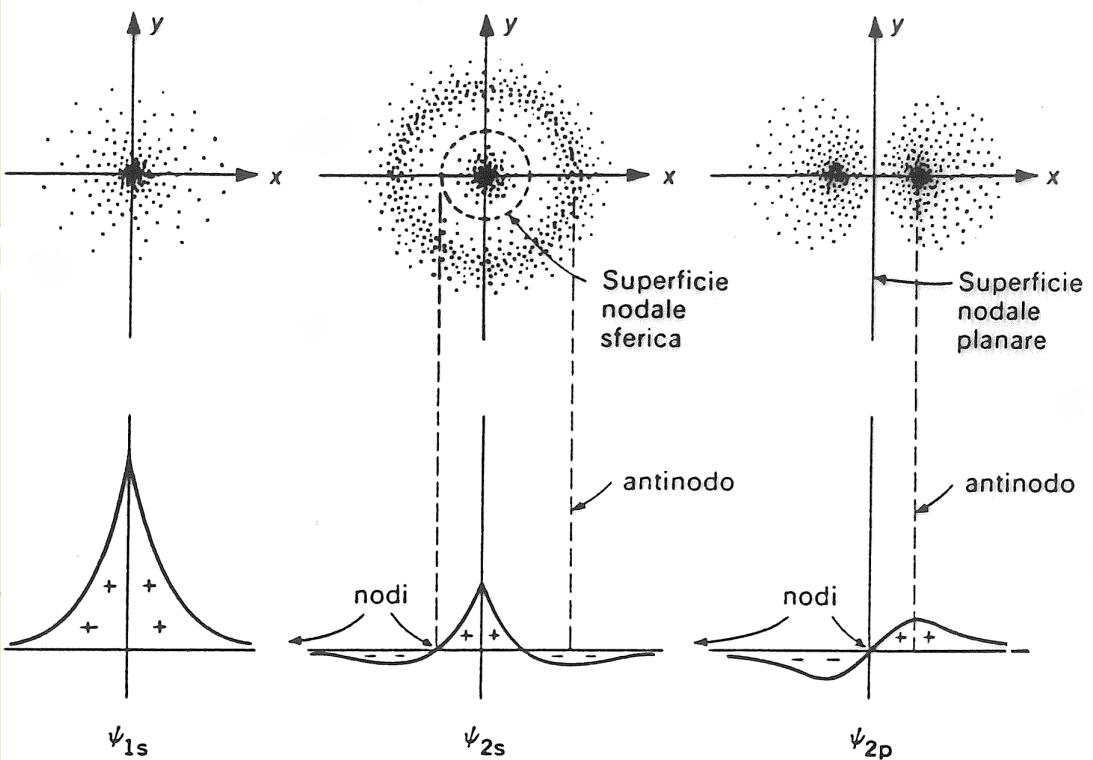
\includegraphics[width=16cm]{immagini/psi.png}
  \caption{Parte radiale}
\end{figure}\\
\begin{itemize}
  \item L'orbitale 1s dell'atomo di idrogeno immagino abbia la forma di un pallone da calcio, dove al centro vi è il nucleo, mentre come superficie esterna del pallone scegliamo la superficie su cui la $\Psi$ vale zero, perché ho immaginato di accontentarmi del 95\% di probabilità di trovare l'elettrone, ed essa per l'orbitale s corrisponde al raggio di questa sfera, che Bohr aveva calcolato essere 0.529 Å.%io ti ammazzo che cazzo metti la virgola, ti ricordo che siamo nel 2022
  
  Quindi per l'orbitale s si ha un andamento tale da immaginarlo come una sfera che contiene l'elettrone, il quale è diffuso all'interno di tutta la sfera.
  \item Il 2s lo immagino con la stessa simmetria dell'1s, solo che stavolta avremo una prima sfera centrata nel nucleo in cui la $\Psi$ è positiva, una superficie nodale e un'altra sfera più grande concentrica alla prima in cui la $\Psi$ è negativa e la cui superficie esterna coincide anche qui col 95\% di probabilità.
  \item Un orbitale 2p lungo un'asse viene rappresentato come due gocce che si uniscono per le due punte. In questo caso al centro il valore della $\Psi$ è zero, mentre nei lobi aumenterà positivamente in uno e negativamente nell'altro.
  \item Un orbitale 3p è simile al 2p, solo che in esso vi è un'altra coppia di lobi che contiene i primi 2 (uno ciascuno).
\end{itemize}
Da notare che se consideriamo solo le superfici più esterne si parla solo di orbitali s e p.

Per quanto riguarda la $\Psi^2$:
\begin{figure}[htp]
  \centering
  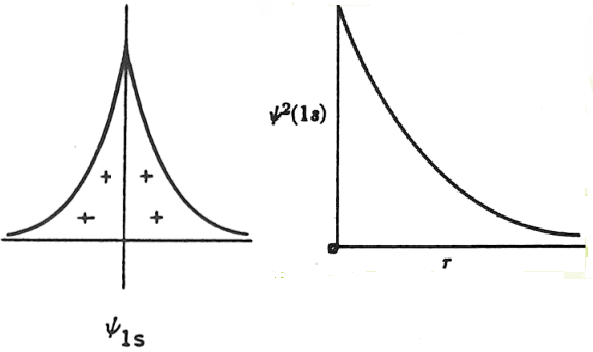
\includegraphics[width=16cm]{immagini/orbitale psi quadro idrogeno.png}
  \caption{Orbitale dell'idrogeno}
\end{figure}\\
\begin{itemize}
  \item Per l'orbitale 1s essa non ha la parte negativa del grafico. Essa ha valore massimo sul nucleo, ma all'aumentare della distanza da questo diminuisce asintoticamente. Anche per essa si taglia al valore in cui abbiamo il 95\% di probabilità, che corrisponderà al raggio dell'orbitale.
\end{itemize}
\textbf{DEF} Si dice probabilità radiale la parte radiale della $\Psi$ al quadrato ($R^2(r)$).

\textbf{DEF} Si dice densità di probabilità radiale l'insieme dei possibili valori del raggio e la relativa probabilità.

Dai grafici prossiamo capire quanto l'elettrone penetri fin dentro il nucleo.

Gli orbitali s penetrano di più nel nucleo rispetto agli altri orbitali, cioè risentono di più della carica nucleare.

Per l'idrogeno i vari orbitali a parità di $n$ sono degeneri, cioè hanno la stessa energia. Ciò non vale più appena aumentano gli elettroni.

Partendo da queste considerazioni si spiega perché in atomi polielettronici gli orbitali s hanno energia più bassa rispetto agli altri.
Moltiplicando il quadrato della funzione d'onda $\Psi^2$ per il volume elementare $dV=4\pi r^2\text{d}r$, è possibile calcolare la probabilità che un elettrone ha di trovarsi in uno spazio sferico definito dallo spessore d$r$ della sfera di raggio r. In particolare, usando la forma $P$d$r$, risulta $P=4\pi r^2\Psi^2$ dove $P$ è la \textbf{funzione di distribuzione radiale}.
\begin{figure}[htp]
  \centering
  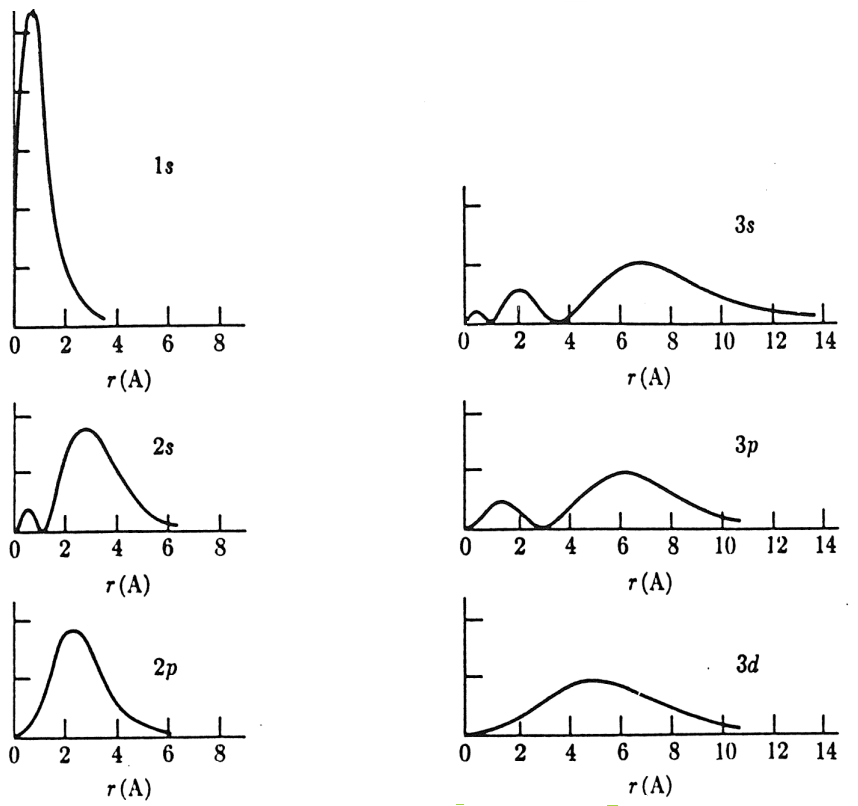
\includegraphics[width=16cm]{immagini/picchi.png}
  \caption{Probabilità di trovare l'elettrone in un guscio sferico, ottenuta dal
  quadrato del modulo della parte radiale dell'orbitale.}
\end{figure}\\
Dovremo quindi ricordare che:
\begin{itemize}
  \item Gli orbitali 3s hanno ulteriori massimi vicino al nucleo oltre quello esterno (sono 3);
  \item Quelli 3p hanno un ulteriore massimo;
  \item I 3d non ne hanno.
\end{itemize}
Siamo soliti descrivere gli orbitali chiudendo ad una data distanza l'orbitale stesso, ossia diamo una dimensione all'orbitale, non lo rappresentiamo come qualcosa di dimensione infinita perché ci accontentiamo che $\Psi^2$ sia 0.95.
%immagini orbitali(colorate)
\begin{itemize}
  \item Forma dell'orbitale s: sferica
  \begin{figure}[htp]
    \centering
    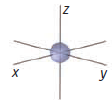
\includegraphics[width=5cm]{immagini/orbitale-s.png}
  \end{figure}\\
  \item Forma dell'orbitale p: due gocce o lobi. Essi sono di segno opposto e il segno segue quello degli assi.
  \begin{figure}[htp]
    \centering
    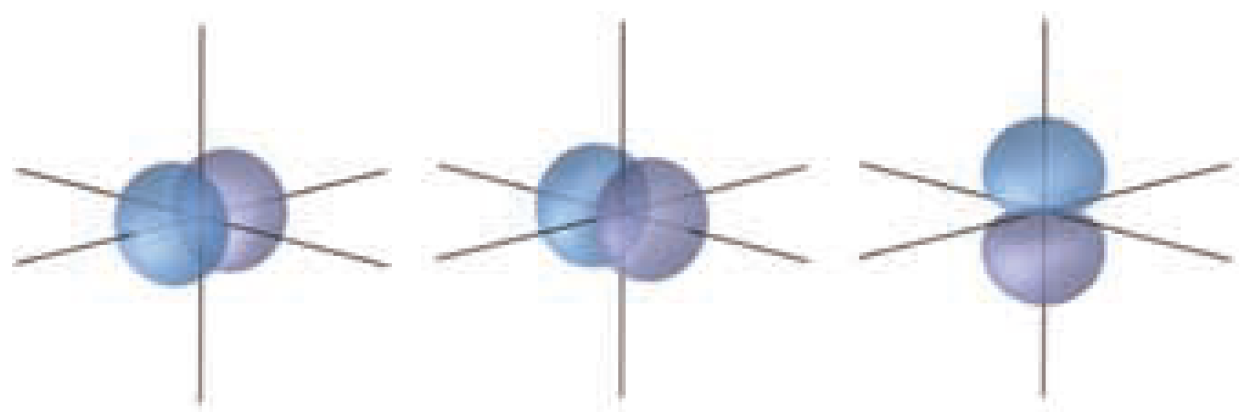
\includegraphics[width=12cm]{immagini/orbitale-p.png}
  \end{figure}\\
  \item Forma degli orbitali d: sono tutti e 5 di forma diversa. Per ognuno di questi orbitali, lobi opposti hanno lo stesso segno.
  \begin{figure}[htp]
    \centering
    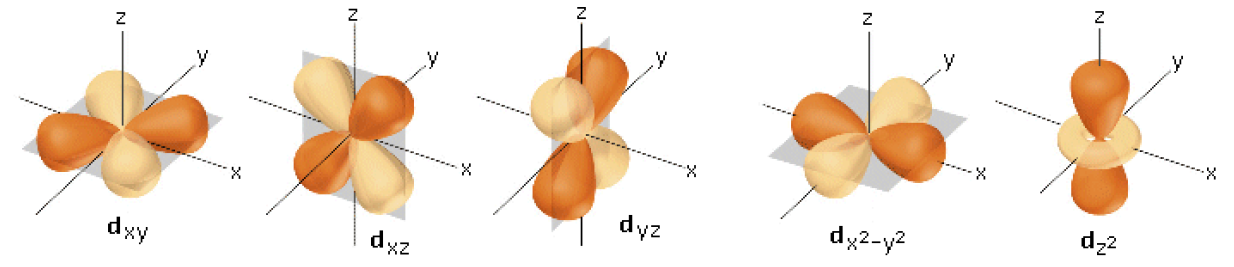
\includegraphics[width=15cm]{immagini/orbitale-d.png}
  \end{figure}\\
  \begin{itemize}
    \item L'orbitale $d_{z^2}$ ha due lobi che giacciono lungo l'asse z, entrambi di segno positivo. Nel piano xy c'è una corona di segno negativo;
    \item L'orbitale $d_{x^2-y^2}$ ha due lobi positivi lungo l'asse x e due lobi negativi lungo l'asse y;
    \item Gli orbitali $d_{xy}$, $d_{xz}$ e $d_{yz}$ hanno lobi che giacciono fra gli assi.
  \end{itemize}
\end{itemize}
Il comportamento di questi orbitali è importante, perché se gli altri leganti puntano lungo gli assi ci saranno sia lobi che puntano direttamente su di essi che lobi che puntano fra di essi.

I piani nelle immagini sono dei nodi perché su di essi la $\Psi$ vale zero e quindi anche la $\Psi^2$, ciòè la probabilità di trovare elettroni è nulla.

Gli orbitali f iniziano a riempirsi nei lantanidi, il primo è il lantanio.

Nell'atomo di idrogeno gli orbitali sono degeneri perché l'energia è funzione solo di $n$.
\subsection{L'influenza della carica nucleare}
\textbf{DEF} Atomi idrogenoidi: atomi che hanno un solo elettrone, così come l'atomo di idrogeno. Per essi siamo capaci di studiarne l'equazione di Schrödinger e capire come influisca il nucleo con la sua carica.

Si osserva che all'aumentare della carica nucleare si contraggono gli orbitali, nonché la parte radiale della $\Psi$.

La carica nucleare fa aumentare drasticamente il potenziale di ionizzazione.

I valori energetici possono essere ottenuti dalla equazione di Schrödinger, correggendola:
$$E=\frac{-313.6(Z^2)}{n^2}=-\frac{RZ^2}{n^2}$$
dove 313.6 è l'energia dello stato fondamentale dell'atomo di idrogeno, che viene indicata anche con la costante di Rydberg $R$. Z è la carica nucleare.

A partire dall'elio ciò non vale più: i valori sperimentali dell'energia non coincidono e gli orbitali 2s e 2p non sono degeneri. Non si hanno quindi soluzioni analitiche.

Supponiamo per assurdo che non ci sia repulsione tra gli elettroni che occupano lo stesso orbitale, in questo caso il valore sperimentale dovrebbe coincidere con quello dato dall'equazione. Ciò che succede nella realtà è che gli elettroni si respingono l'un l'altro, destabilizzando il sistema (più è negativa l'energia, più stabile sarà il sistema) e pertanto è più facile strappare un elettrone (ricorda: l'energia di un elettrone in un dato orbitale è misurabile dal potenziale di ionizzazione di quell'orbitale). Ciò dipende dal fatto che gli elettroni non amano stare nello stesso orbitale, si respingono l'un l'altro in quanto aventi cariche dello stesso segno e per questo motivo il sistema è destabilizzato.
\subsection{Sequenza energetica dell'atomo di idrogeno}
\begin{itemize}
  \item 1s più vicini al nucleo ed energia più negativa.
  \item 2s e 2p degeneri (4 totali).
  \item 3s, 3p e 3d degeneri (1s+3p+5d=9 livelli).
\end{itemize}
Quando abbiamo a che fare con più elettroni questi livelli si separeranno in energia. Il motivo è che ci sono orbitali, cioè funzioni d'onda, che penetrano più vicino il nucleo, quindi gli elettroni che li occupano sentiranno l'intera carica nucleare, mentre orbitali più esterni, che penetrano meno nel nucleo, se occupati vedranno elettroni che sentono una carica nucleare inferiore, perché c'è un'azione di schermaggio da parte degli elettroni interni. Essendo meno legati, la loro energia è minore in valore assoluto.
\subsection{La carica efficace}
Con atomi polielettronici non c'è più la degenerazione dei livelli a parità di numero quantico principale, ma l'energia oltre che da n dipenderà anche da l.\\

Ricorda: l'energia di un elettrone in un dato orbitale  equivale all'energia necessaria per strappare questi elettroni e ionizzare l'atomo usando l'equazione di Einstein per interpretare l'effetto fotoelettrico (inviamo una certa energia, misuriamo l'energia cinetica degli elettroni emessi e la differenza sarà il potenziale di ionizzazione. (Approssimazione di Koopmans: l'energia dell'elettrone di un orbitale è pari all'energia richiesta per ionizzare quegli elettroni))\\

Per l'atomo di elio si ottiene, dall'equazione corretta, un potenziale di ionizzazione di -1254.4 Kcal/mol per l'orbitale 1s, mentre sperimentalmente si trova un valore di -567 Kcal/mol. Com'è possibile?

Si pensa subito al fatto che a causa della presenza di due elettroni nello stesso orbitale ci sia una forte energia repulsiva che destabilizza il sistema. Tale termine repulsivo non permette di risolvere l'equazione di Schrödinger.

Cerchiamo quindi di correggere ulteriormente l'equazione mettendo, al posto della carica Z, la carica effettiva o efficace Z$^*$. Ciò in pratica corrisponde al partire dal valore sperimentale osservato per valutare Z$^*$:
$$E=\frac{-313.6(Z^{*2})}{n^2} \implies -567.7=-313.6\frac{Z^{*2}}{1} \implies Z^*=1.34$$
Noi invece ci aspettavamo Z=2, perché nell'elio abbiamo 2 protoni. La carica quindi risulta inferiore. Ciò significa che gli elettroni si schermano a vicenda dalla carica nucleare, e quindi anziché sentire la carica nucleare di 2 protoni ne avvertono una inferiore, pari a 1.34 protoni, quindi risultano meno legati.\\

Ciò vale per lo stato fondamentale dell'atomo di elio. Consideriamo altri 2 casi in cui gli elettroni hanno spin paralleli.

Se costringiamo il sistema, pur avendo elettroni in orbitali diversi, ad accoppiare lo spin, il sistema sarebbe ancora meno stabile. Si dice che un sistema con elettroni spaiati tende ad avere la massima molteplicità di spin, ossia tende ad avere gli spin paralleli. Se pensiamo di accoppiare due spin in orbitali diversi spendiamo energia.
Due elettroni con spin diverso non possono essere scambiati, due elettroni con lo stesso spin invece si. Poter scambiare gli elettroni abbassa l'energia.

Per gli orbitali 2s e 2p, con i valori sperimentali dell'energia si ottengono valori di Z$^*$ pari rispettivamente a 1.08 e 0.997 protoni, quindi l'elettrone 2s è fortemente schermato dalla carica nucleare dall'elettrone 1s, tant'è che sente poco più di 1 protone. Analogamente per l'elettrone 2p.

Si deduce che la carica nucleare sentita dagli elettroni esterni è inferiore rispetto al valore totale, perché gli elettroni interni schermano questi dall'influenza della carica nucleare. Diventa quindi chiaro capire perché serve sapere quali orbitali sono stati occupati oltre quello esterno, perché se strappo elettroni inizio strappando quelli più esterni, la cui energia dipende anche da quali altri orbitali interni sono occupati in quanto sarà più o meno schermato.

L'energia pertanto non dipende più solo dal numero quantico principale $n$, ma dipende sia da $n$ che da $l$.

\begin{figure}[htp]
  \centering
  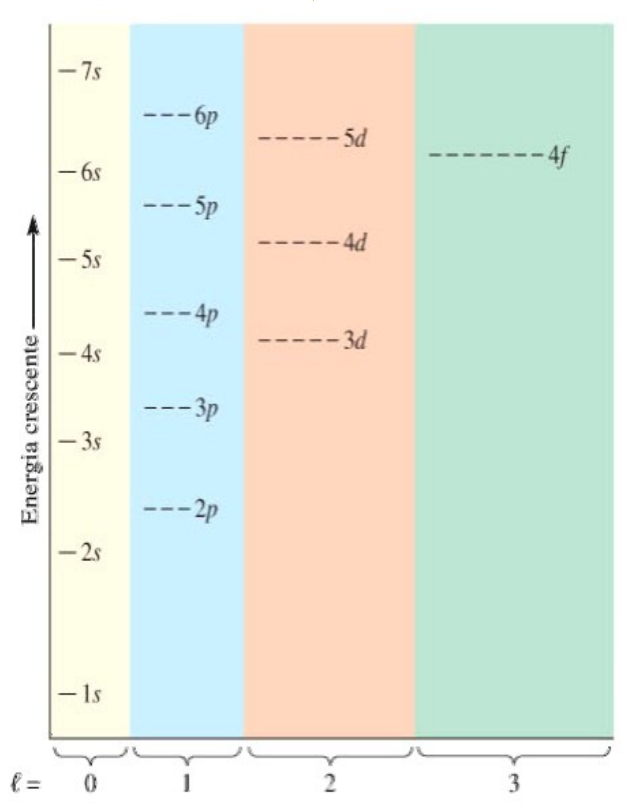
\includegraphics[width=12cm]{immagini/livelli orbitali.png}
  \caption{Ordine di occupazione degli orbitali}
\end{figure}
La differenza nella capacità di penetrazione determina la separazione in energia degli orbitali s, p, d ed f a parità numero quantico principale negli atomi polielettronici.

Quando $n$=3 si riempiono i livelli 3s e poi i 3p. Dopo ci aspetteremmo che l'elettrone successivo vada negli orbitali 3d, ma non è così.

Consideriamo l'argon. Con i suoi 18 elettroni si raggiunge la configurazione elettronica fatta così: 1s, 2s, 2p, 3s, 3p.

Se passiamo al potassio che ha 19 elettroni, seguendo la logica di quella sequenza si penserebbe che ospiti il 19° elettrone in orbitali 3d (che in teoria sono quelli immediatamente disponibili dopo aver riempito i 3p) perché a stesso numero quantico, ma non è così: lo osserviamo nel 4s, lasciando quindi vuoti i 5 orbitali 3d.

Il motivo per cui si riempie prima tale livello, è che la sua densità di probabilità radiale ha un massimo principale più esterno rispetto al 3d, ma gli ulteriori massimi sono a distanze prossime a quelle del nucleo, pertanto gli elettroni 4s sentiranno l'intera carica nucleare molto di più di quanto la sentano gli elettroni 3d, e in conseguenza a ciò i 4s si riempiono prima dei 3d perché questi risentono di più del passaggio da 18 protoni nell'argon a 19 nel potassio e quindi si stabilizzano prima. Affinché la carica nucleare faccia abbassare in energia i livelli 3d si deve arrivare allo scandio, col quale si stabilizzano e iniziano a riempirsi. Quando saranno riempiti (con lo zinco) si tornerà agli orbitali col numero quantico 4, ossia ai 4p.

L'ordine con cui si riempiono gli orbitali è quindi 3p, 4s, 3d e 4p.

Questa anomalia si ripercuote sui 4d, 5d, 4f, 5f ecc.

Gli effetti di questa sequenza energetica di orbitali sono
\begin{itemize}
  \item La capacità di penetrazione di alcuni orbitali più vicino al nucleo tanto da risentire dell'intera carica nucleare molto più di quanto non accada per livelli a numero quantico inferiore ma che non hanno massimi in prossimità del nucleo.
  \item Lo schermaggio degli elettroni interni nei confronti di quelli esterni dall'influenza della carica nucleare.
\end{itemize}
Va da ricordare che vige il principio di esclusione di Pauli, che afferma che un orbitale non può contenere più di due elettroni, per cui:
\begin{itemize}
  \item Gli orbitali s possono contenere 2 elettroni
  \item Gli orbitali p possono contenere 6 elettroni
  \item Gli orbitali d possono contenere 10 elettroni
  \item Gli orbitali f possono contenere 14 elettroni
\end{itemize}
Gli atomi che contengono elettroni di tipo 4f si chiamano lantanidi. Prendono il nome dal primo elemento con elettroni di questo tipo, il lantanio.

Gli atomi che contengono elettroni di tipo 5f si chiamano lantanidi. Prendono il nome dal primo elemento con elettroni di questo tipo, l'attinio.
\newpage
\subsection{Notazione per la funzione d'onda}
\begin{figure}[htp]
  \centering
  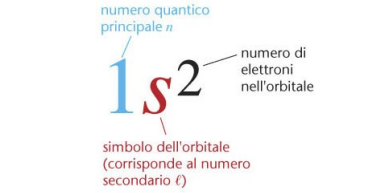
\includegraphics[width=12cm]{immagini/notazione.png}
\end{figure}
In questo caso con questa notazione stiamo dicendo che abbiamo due elettroni nell'orbitale 1s.

\subsection{Alcune configurazioni elettroniche (perlopiù elementi di transizione)}
Gli elementi di transizione hanno orbitali d parzialmente occupati. Ne segue che zinco, cadmio e mercurio non sono elementi di transizione perché completano i livelli d. L'ultimo elemento di transizione è il rame.
\begin{itemize}
  \item Il potassio mostra un elettrone 4s e i 3d sono vuoti.
  \item Il calcio ha due elettroni 4s e i 3d sono vuoti.
  \item Lo scandio ha due elettroni 4s e il primo elettrone 3d (è il primo elemento di transizione).
  \item Il titano ha due elettroni 4s e il secondo elettrone 3d (4s$^2$ 3d$^2$).
  \item Il vanadio ha configurazione elettronica 4s$^2$ 3d$^3$.
  \item Il cromo anziché avere configurazione elettronica 4s$^2$ 3d$^4$ mostra una configurazione 4s$^1$ 3d$^5$. Questo perché gli orbitali d sono 5, e le configurazioni elettroniche d$^0$ (nessun elettrone d), d$^5$ (un elettrone per ogni orbitale) e d$^{10}$ (orbitali d totalmente pieni) sono altamente stabili, quindi il cromo preferisce spostare un elettrone dai 4s ai 3d. Quello che succede è che un elettrone salta: mentre fino al vanadio avevamo l'orbitale 4s pieno, ora si svuota parzialmente in modo tale che i 6 elettroni figurino uno sull'orbitale s e 5 sul d.
  \item Il manganese ha configurazione 4s$^2$ 3d$^5$.
  \item Il ferro ha configurazione 4s$^2$ 3d$^6$.
  \item Il cobalto ha configurazione 4s$^2$ 3d$^7$.
  \item Il Nichel ha configurazione 4s$^2$ 3d$^8$.
  \item Il rame, anziché mostrare configurazione 4s$^2$ 3d$^9$, sposta un elettrone di tipo s per riempire tutti gli orbitali d e arrivare quindi a d$^{10}$, ed ha quindi una configurazione elettronica 4s$^1$ 3d$^{10}$.
\end{itemize}
Le anomalie del cromo e del rame sono quindi dovute alla propensione ad avere gli orbitali d, rispettivamente, tutti singolarmente occupati e tutti pieni. Preferiscono dunque creare una lacuna negli orbitali 4s.

Questo fenomeno si ripete nel gruppo zinco, cadmio e mercurio e in quello cromo, molibdeno e tungsteno.